% =====================================================================
%  Anchor Recycling — Elsevier elsarticle build
%  Source of truth: ../paper_manuscript_v1.md (v1.0, 2026-11-21)
%  Build:  pdflatex main && pdflatex main   (no BibTeX; thebibliography)
%  TODO before submission: fill author list / affiliation / journal.
% =====================================================================
\documentclass[preprint,12pt,number]{elsarticle}

\usepackage[T1]{fontenc}
\usepackage[utf8]{inputenc}
\usepackage{mathptmx} % Times-like text+math; newtx hangs on this MiKTeX install
\usepackage{amsmath,amssymb}
\usepackage{graphicx}
\usepackage{booktabs}
\usepackage{array}
\usepackage{float}
\usepackage[font=small,labelfont=bf]{caption}
\usepackage{microtype}
\usepackage{url}
\usepackage[colorlinks=true,allcolors=blue!45!black]{hyperref}

\graphicspath{{../figures/}}
\setcitestyle{numbers,sort&compress}
\setlength{\emergencystretch}{2em}

% Shorter, journal-style section spacing in preprint mode
\setlength{\abovecaptionskip}{6pt}
\setlength{\belowcaptionskip}{2pt}

\journal{Pattern Recognition Letters}

\begin{document}

\begin{frontmatter}

\title{Anchor Recycling: Label-Efficient Skeleton Behavior Recognition Under Evolving Taxonomies}

% TODO: replace with the author block before submission.
\author[1]{Anonymous Authors}
\affiliation[1]{organization={Affiliation to be completed}, country={Country}}

\begin{abstract}
Skeleton behavior recognition under evolving taxonomies faces a recurring
constraint: label taxonomies and domains keep changing while annotation
budgets stay small. Decoupled frameworks that freeze a self-supervised physical layer and
adapt only a semantic layer preserve label efficiency, but they cap
performance in \emph{weak-reference tiers} where labels are few, noisy, or
indirectly derived. Through a controlled four-tier study (NTU60 $\rightarrow$ PanAf500 $\rightarrow$
NTU120 $\rightarrow$ UCF101) governed by a single measurement implementation, we first map
this ceiling and then, on the NTU120 tier, test four label-free routes around
it: test-time entropy minimization, low-rank continued pretraining,
cross-domain transfer from a strong source, and pseudo-label feedback. All
four fail: no route gains more than $+0.1$~pp, and none of them supplies label
signal to the encoder. We then show that the ceiling can be raised: the \emph{same} small anchor set
that drives the semantic layer can be \textbf{recycled} to shape the physical layer
through low-rank supervised adaptation with a distillation anchor. Anchor
recycling improves budget-limited retention by $+10.20$~pp on NTU120 (74.96\% $\rightarrow$
85.16\%, PARTIAL), $+9.71$~pp on PanAf500 (82.50\% $\rightarrow$ 92.21\%, CONFIRMS), and $+20.12$
pp on UCF101 (51.09\% $\rightarrow$ 71.21\%), the largest gain appearing on the
weakest-reference tier. The effect has a two-sided envelope: a minimum anchor mass below
which unaugmented adaptation is inert, and a calibration gate above which the semantic
layer refuses the adapted features. We map both axes across tiers, with a
unimodal response to augmentation peaking at 85.16\%. We release the unified
measurement harness and all per-seed evidence.
\end{abstract}

\begin{keyword}
skeleton-based action recognition \sep label-efficient learning \sep
parameter-efficient adaptation \sep self-supervised pretraining \sep
evolving taxonomies
\end{keyword}

\end{frontmatter}

% =====================================================================
\section{Introduction}
% =====================================================================

Skeleton-based action recognition has matured on benchmarks with abundant,
clean labels. Deployed systems rarely enjoy that luxury. The label taxonomy
itself evolves (classes are merged, renamed, split, or added as a deployment
reveals what actually matters), and new domains arrive with little in-domain
supervision because the annotations must be produced by scarce domain
experts. A recognition framework intended for this reality must therefore be
judged by how much of its full-label accuracy it \emph{retains} as the budget
shrinks and the reference degrades.

The physics--semantics decoupling (PSD) framework was designed for exactly
this regime. A self-supervised \textbf{physical layer} (an AimCLR-style~\cite{aimclr}
contrastive pretext over skeletons) is frozen after pretraining; a
\textbf{semantic layer} (rule-based seed extraction, anchor clustering,
confidence-filtered pseudo-labels, and a self-training head) adapts to the
current taxonomy using only a small stratified anchor set. The framework is judged by a
pre-registered \emph{budget-retention protocol}: the ratio of the small-budget
pipeline accuracy to the full-label linear-probe accuracy of the same frozen
encoder, with verdict bands CONFIRMS ($\ge 90\%$), PARTIAL (85--90\%), and FAILS
($<85\%$). It confirms its label-efficiency claim on the strong-reference
tier NTU60 (90.7\% retention at a 10\% budget). On weak-reference
tiers, however, it hits a ceiling: 82.50\% on the chimpanzee behavior tier
PanAf500, 74.96\% on the 60-class NTU120 subset, and 51.09\% on UCF101
skeletons.

This paper is about that ceiling, and about the natural hypothesis that
adapting the encoder should close the gap. We first test whether the encoder
can be adapted \emph{for free}, without spending any additional labels,
and answer negatively with a systematic negative-result study. On the NTU120
tier we evaluate four families of label-free adaptation: (i) test-time
entropy minimization over BatchNorm affine parameters; (ii) low-rank
continued self-supervised pretraining on all unlabeled target clips; (iii)
cross-domain transfer, initializing from a strong NTU60 source encoder and
adapting to the weak target; and (iv) pseudo-label feedback, using the
semantic layer's own confidence-gated pseudo-labels to retrain the encoder
with supervised contrastive learning. Every family leaves budget-limited
retention within $+0.1$ to $-5.2$~pp of the frozen baseline. The ceiling persists
because \emph{true label signal never reaches the encoder}.
Each failure mode helps to explain this conclusion,
from a BatchNorm statistics trap to a feature-geometry/harvest mismatch.

The positive contribution follows directly from the diagnosis. The semantic
layer already consumes a small stratified anchor set; we \textbf{recycle those
identical anchors} as supervision for a low-rank update of the physical
layer. A fresh linear head and LoRA adapters (3.19\% of parameters,
zero-initialized so adaptation starts exactly at the frozen solution) are
trained on the anchor clips with cross-entropy plus a cosine distillation
anchor to the frozen encoder, while BatchNorm running statistics remain
frozen to keep the train/evaluation feature contract intact. The adapted
encoder re-enters the \emph{same} three-arm protocol, measured by the \emph{same}
implementation. We call this \textbf{anchor recycling}: a second use of labels
that already existed.

Anchor recycling delivers consistent gains across the three weak-reference
tiers: $+10.20$~pp on NTU120 (74.96\% $\rightarrow$ 85.16\%, crossing into the PARTIAL
band), $+9.71$~pp on PanAf500 (82.50\% $\rightarrow$ 92.21\%, crossing into CONFIRMS), and
$+20.12$~pp on UCF101 (51.09\% $\rightarrow$ 71.21\%). A budget-allocation sweep shows the
advantage widens with budget ($+2.90$~pp at 5\%, $+3.91$~pp at 10\%, $+4.56$~pp at 15\%),
and a hyperparameter study isolates the adaptation learning rate and the
anchor-augmentation multiplier as the dominant factors, with a unimodal
response to augmentation peaking at $\times 8$ (85.16\%) and a hard calibration-gate
boundary at high pressure.

Our contributions are:

\begin{enumerate}
\item \textbf{A weak-reference evaluation protocol} for skeleton recognition under
  evolving taxonomies: four tiers of graded reference quality, a fixed
  budget-retention protocol implemented once and shared by every number in the
  paper, and pre-registered verdict bands.
\item \textbf{A systematic negative-result study} establishing that four families of
  label-free encoder adaptation cannot close the weak-reference gap, with
  mechanism-level diagnostics (a BatchNorm train/eval statistics trap, a
  feature-geometry/harvest mismatch, and label inheritance) that explain
  \emph{why} each route fails.
\item \textbf{Anchor recycling}, a label-efficient adaptation mechanism that reuses
  the semantic layer's anchor set to shape the physical layer, yielding
  $+10.2/+9.7/+20.1$~pp on three weak-reference tiers and crossing two
  pre-registered verdict bands.
\item \textbf{A two-sided envelope analysis} (an anchor-mass floor and a
  calibration-gate ceiling), together with a sensitivity map over
  augmentation, learning rate, and budget that separates configurations
  that improve retention from those that leave it unchanged or trip the
  calibration gate.
\end{enumerate}

% =====================================================================
\section{Related Work}
% =====================================================================

\subsection{Self-supervised skeleton pretraining}

Contrastive and masked-prediction pretexts build strong physical
representations without labels: AimCLR~\cite{aimclr} contrasts extreme augmentations of
the same clip with a momentum queue; CrosSCLR~\cite{crossclr} extends contrast to
cross-stream views; hBehaveMAE~\cite{hbehavemae} and similar masked-autoencoder approaches
learn spatio-temporal recovery for animal behavior; TREBA~\cite{treba} applies
temporally guided self-supervision to 3D human pose and action recognition;
and ProSL~\cite{prosl} progressively refines cluster-level pseudo-labels for
unsupervised skeleton action recognition. These
skeleton pretexts descend from a broader vision lineage of contrastive and
self-distilled pretraining~\cite{moco,simclr,byol,clip,dinov2}, built on the representations and
architectures of large-scale image learning~\cite{alexnet,resnet}. Our physical layer
follows the AimCLR single-stream joint recipe at
reduced capacity (16 hidden channels, 1.84\,M parameters), chosen so that
every tier is computable under one protocol. Our study concerns the stage
that follows pretraining: \emph{what should happen when the taxonomy and the
budget change} --- a question prior work does not answer.

\subsection{Domain and test-time adaptation}

Source-free and test-time adaptation methods update a model on unlabeled test
data: TENT~\cite{tent} minimizes prediction entropy over BatchNorm affine parameters,
and a family of related methods~\cite{dann,bendavid,tta_distmatch,bituning} adapts normalization statistics or
low-capacity parameters online. We adopt TENT as one of four label-free
adaptation baselines and find that, once the BatchNorm train/evaluation
statistics contract is made consistent, test-time adaptation has little
effect on skeleton features under a weak reference: the feature geometry,
not its calibration, is the constraint.

\subsection{Continual and class-incremental learning under taxonomy change}

Taxonomy evolution of this kind is studied in class-incremental and
continual learning. Knowledge distillation preserves old-class behavior while
learning new classes (LwF~\cite{lwf}; distillation~\cite{distillation}). Prior work in our
framework~\cite{prior} established a zero-retraining bound for merge/rename events (76.8\%
oracle / 76.5\% argmax-voting on an NTU60$\rightarrow$10-class merge) and an adaptation
ladder for split/addition (remap 0\% $\rightarrow$ decoupled 45.75\% $\rightarrow$ frozen 68.05\% $\rightarrow$
coupled 97.13\%). In this paper we use LwF as an adapted class-incremental
baseline at matched budget (68.6\% at the 10\% budget on the TRANS-002 merge ---
the pre-registered NTU60 60$\rightarrow$49 taxonomy-transition episode of our prior
study~\cite{prior}, distinct from the 60-class NTU120 subset of \S4; 72.9\% at full labels)
and show that anchor recycling is orthogonal to distillation-based
incremental schemes.

\subsection{Label-efficient learning}

Semi-supervised and self-training methods~\cite{entropy_min,pseudolabel,fixmatch} amplify small anchor sets
with pseudo-labels; supervised contrastive learning (SupCon~\cite{supcon}) structures
representations with label supervision; LoRA~\cite{lora} provides parameter-efficient
adaptation originally formulated for language models. These adapters rest on
standard optimization and regularization components --- AdamW~\cite{adamw} and Adam~\cite{adam}
among the optimizers, dropout~\cite{dropout} among the regularizers --- while data
augmentation~\cite{augmentation} is the standard lever for enlarging a small labeled set,
the role it plays in \S3.2. Multi-task learning~\cite{multitask} is the classical
precedent for sharing one representation across tasks; earlier skeleton
pipelines instead paired hand-crafted features with classifiers such as
random forests~\cite{randomforest}. Our negative-result
study applies pseudo-label feedback and SupCon to the encoder itself and
shows they cannot substitute for true labels in the weak-reference regime.
Our positive method combines LoRA with supervised anchors; the contribution
lies in the \emph{demonstration that the same anchor set must supervise both
layers of a decoupled pipeline}, and in the mapping of the envelope in which
this holds.

\subsection{Positioning}

None of the above studies the weak-reference regime with a fixed
budget-retention protocol across four tiers of graded reference quality, and
none asks which layer of a decoupled framework should receive the labels.
Prior transferability analyses~\cite{yosinski,transfer_survey} address representation transfer, not
label allocation between the layers of a decoupled pipeline. That question,
and its two-sided answer, is the subject of this paper.

% =====================================================================
\section{Method}
% =====================================================================

\subsection{Preliminaries: the decoupled framework and its protocol}

The PSD framework separates a \textbf{physical layer} from a \textbf{semantic layer}.
The physical layer is a self-supervised AimCLR pretext (ST-GCN~\cite{stgcn} base, 16
hidden channels, 1.84\,M parameters before the low-rank adaptation of \S3.2,
150 epochs, single-stream joint), frozen
after pretraining. The semantic layer adapts to the current taxonomy from a
small stratified anchor set through rule-based seed extraction, anchor
clustering, confidence-filtered pseudo-labeling, and a self-training
classification head.

The evaluation protocol measures \textbf{budget retention}: with a stratified
$b$\% anchor draw (seeds 42--51), the pipeline's validation accuracy is divided
by the full-label linear-probe accuracy of the same frozen encoder (logistic
regression via scikit-learn~\cite{sklearn}). Verdict
bands are pre-registered: retention $\ge 90\%$ CONFIRMS, 85--90\% PARTIAL, $<85\%$
FAILS. All numbers in this paper are produced by one shared implementation of
the three arms: (a) $b$\% linear head, (b) $b$\% + semantic pipeline, and (c)
full-label linear reference, so that cross-tier and cross-paper comparisons
use a single protocol.

\subsection{Anchor recycling}

Given the anchor set $A$ ($|A| = b\%$ of the training clips, drawn exactly as
the semantic layer's anchors), anchor recycling performs a low-rank
supervised update of the physical layer before the semantic stage:

\textbf{Step 1 --- Low-rank injection.} Every Conv2d in the query encoder receives a
parallel LoRA branch (rank $r = 8$, $\alpha = 16$): $y = \mathrm{conv}(x) + (\alpha/r)\,B(A(x))$,
with $B$ zero-initialized so that the adapted encoder is functionally
identical to the frozen one at step zero. The key encoder receives the same
injection and is momentum-synced; the contrastive machinery is unused during
recycling. Trainable parameters: 62,616 of 1,965,368 (3.19\%); the 62,616 are
the LoRA branches of the query encoder, the only parameters the optimizer
updates, while the key encoder's identical branches are momentum-synced and
not optimizer-trainable. The 1.84\,M figure refers to the frozen base encoder
before injection.

\textbf{Step 2 --- Objective.} Cross-entropy on the anchor clips through a fresh
linear head ($256 \rightarrow C$), plus a cosine feature distillation anchor
$1-\cos(f_s, f_t)$ between the adapted and frozen encoder features,
weighted by $\lambda$. BatchNorm~\cite{batchnorm} running statistics are frozen (the encoder is kept
in evaluation mode during adaptation) so that the features seen during
adaptation match the features later exported for the semantic stage; this
consistency requirement comes from the test-time adaptation diagnostics
in \S4.2.

\textbf{Step 3 --- Anchor augmentation.} When anchor mass is small, each epoch
samples $V\times|A|$ augmented views of the anchors through the pretext's own
augmentation family (shear amplitude 0.5, temporal padding ratio 6), turning
even a 40-anchor set into hundreds of distinct gradient signals without new
labels. The multiplier $V$ is a tier-dependent hyperparameter mapped in \S4.5.

\textbf{Step 4 --- Re-measurement.} The adapted encoder is frozen, features are
re-exported, and the identical three-arm protocol is re-run, including a
fresh full-label linear reference, so the denominator reflects the adapted
encoder.

No additional labels are used anywhere in this pipeline: the recycling stage
sees exactly the anchor set that the semantic stage already consumes.

\subsection{The calibration gate}

The semantic layer includes a calibration gate: a step that selects a
similarity threshold $\tau$ from a candidate grid and rejects degenerate
calibrations~\cite{rejection}. We
found this gate to be an unexpected safety mechanism during encoder
adaptation: when recycling pressure is too strong, the adapted feature
geometry drives the selected $\tau$ to zero and the pipeline raises a hard error
instead of producing degenerate pseudo-labels. \S4.6 maps this gate as the
upper bound of the adaptation envelope.

% =====================================================================
\section{Experiments}
% =====================================================================

\subsection{Setup}

Four tiers are ordered by reference quality: NTU60~\cite{ntu60} (published retention
90.7\%), PanAf500~\cite{panaf20k} (82.50\%), NTU120~\cite{ntu120} (74.96\%), and UCF101~\cite{ucf101}
(51.09\%). Each has
its own from-scratch label-free pretext (150 epochs) and a 10\% stratified
anchor budget (seeds 42--51; ten seeds for every headline number). NTU120's
anchors number 734, UCF101's 953, and PanAf500's 40; this spread, together
with reference quality, shapes the adaptation envelope (\S4.5--4.6). Figure~\ref{fig:four-tier}
shows the resulting four-tier gradient of budget retention.

\begin{figure}[t]
\centering
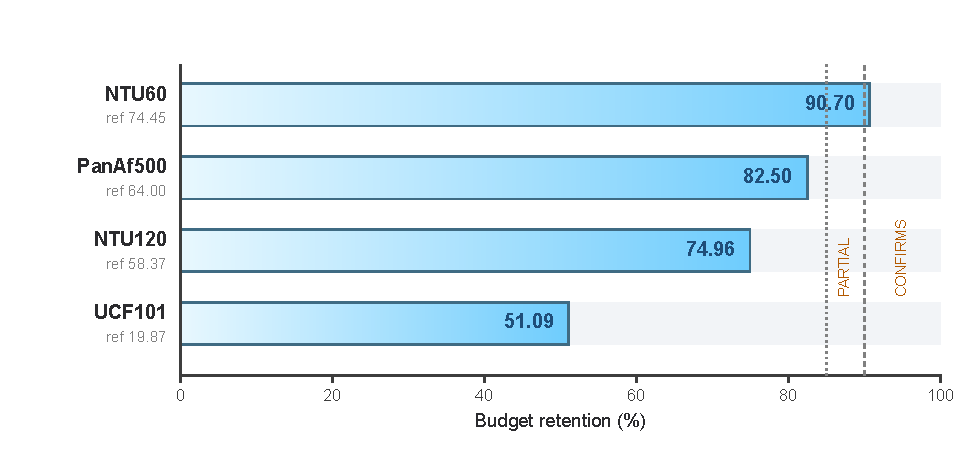
\includegraphics[width=\linewidth]{fig1_four_tier_gradient.pdf}
\caption{Four-tier gradient of budget retention (10\% anchors). Bars give
each tier's retention on a common 0--100 scale; the grey label under each tier name
gives the full-label linear-probe accuracy that defines its denominator.
Vertical lines mark the 85\% and 90\% verdict thresholds (PARTIAL and CONFIRMS).}
\label{fig:four-tier}
\end{figure}

\subsection{Zero-label adaptation does not move a frozen physical layer}

We test four label-free adaptation families on NTU120, the tier with the most
complete instrumentation; the cross-domain family is instantiated as two
arms (zero-shot transfer and LoRA transfer), giving the five adaptation rows
of Table~\ref{tab:labelfree}:

\begin{table}[t]
\centering
\caption{Label-free adaptation arms on the NTU120 tier (10\% budget).}
\label{tab:labelfree}
\begin{tabular}{@{}lrr@{}}
\toprule
Arm & Retention & $\Delta$ vs.\ frozen \\
\midrule
Frozen baseline                         & 74.96\% & --- \\
TENT (BN affine, eval-statistics)       & 74.08\% & $-0.88$~pp \\
Same-domain LoRA continued pretraining  & 74.99\% & $+0.03$~pp \\
Cross-domain zero-shot (NTU60 $\rightarrow$ NTU120) & 69.77\% & $-5.19$~pp \\
Cross-domain LoRA transfer              & 71.98\% & $-2.98$~pp \\
Pseudo-label SupCon feedback            & 74.98\% & $+0.02$~pp \\
\bottomrule
\end{tabular}
\end{table}

Three diagnostics explain these failures.

First, a naive TENT setup that adapts in BatchNorm train mode collapses to
27.0\%, entirely a train/evaluation statistics artifact; once the statistics
contract is fixed, TENT shifts retention by only $-0.88$~pp (74.96\% $\rightarrow$ 74.08\%).

Second, same-domain continued pretraining is saturated: the from-scratch
pretext has already consumed its own data for 150 epochs, and 30 further
low-rank epochs change nothing.

Third, cross-domain transfer produces the \emph{best absolute separability} of any
arm: the full-label linear reference rises to 59.66\% (vs.\ 58.37\% frozen) and
the 10\% linear head to 45.27\% (vs.\ 44.18\%), yet retention \emph{falls} to
71.98\%. The semantic layer's anchor clustering was grown around the frozen
geometry and cannot harvest the improved features: improving the features is
feasible, but the binding constraint is whether the pipeline's discrete
stages can absorb the improvement.

Pseudo-label feedback closes the loop in the other direction, retraining
the encoder with the semantic layer's own pseudo-labels via SupCon over 7,239
covered samples, and fares no better (74.98\%). Pseudo-labels inherit the frozen encoder's
geometry; feeding them back reinforces it rather than repairing it.

\begin{quote}
\textbf{Finding 1.} Four label-free adaptation families (spanning test-time,
self-supervised, cross-domain, and semi-supervised mechanisms) move
budget-limited retention by at most $+0.1$~pp and as much as $-5.2$~pp. The
weak-reference ceiling is structural: it is the absence of true label signal
at the encoder, not a lack of adaptation capacity.
\end{quote}

\subsection{Anchor recycling: main results}

Recycling the semantic layer's anchors into the physical layer with per-tier
optimal settings (\S4.5) yields the per-tier main results in Table~\ref{tab:main}, plotted
in Figure~\ref{fig:main}:

\begin{table}[t]
\centering
\caption{Anchor recycling main results per tier (10\% budget; per-tier
optimal settings of \S4.5).}
\label{tab:main}
\footnotesize
\setlength{\tabcolsep}{4pt}
\begin{tabular*}{\textwidth}{@{\extracolsep{\fill}}lrr>{\raggedright\arraybackslash}p{2.65cm}r@{\hspace{10pt}}>{\raggedright\arraybackslash}p{1.95cm}@{}}
\toprule
Tier & Anchors / budget & Frozen & Recycling & $\Delta$ & Verdict \\
\midrule
NTU120   & 734 / 10\% & 74.96\% & \textbf{85.16\%}\newline (lr 2e-2, aug $\times 8$) & \textbf{+10.20}~pp & FAILS$\to$\newline\textbf{PARTIAL} \\
PanAf500 & 40 / 10\%  & 82.50\% & \textbf{92.21\%}\newline (lr 1e-2, aug $\times 4$) & \textbf{+9.71}~pp  & FAILS$\to$\newline\textbf{CONFIRMS} \\
UCF101   & 953 / 10\% & 51.09\% & \textbf{71.21\%}\newline (lr 2e-2)               & \textbf{+20.12}~pp & FAILS$\to$\newline FAILS \\
\bottomrule
\end{tabular*}
\end{table}

\begin{figure}[t]
\centering
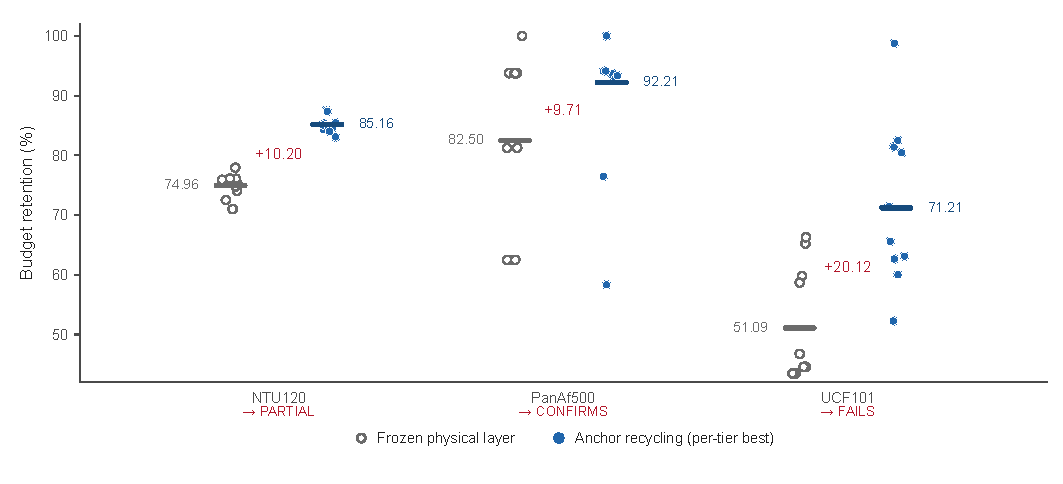
\includegraphics[width=\linewidth]{fig2_tier_main_results.pdf}
\caption{Per-tier main results of anchor recycling at the 10\% budget
(Table~\ref{tab:main}). Each panel shows one tier: thin grey lines are individual seeds
($n = 10$), the thick line runs from the frozen mean to the recycled mean, and
the gain and post-recycling verdict are printed with the panel. NTU120 74.96\%
$\rightarrow$ 85.16\%, PanAf500 82.50\% $\rightarrow$ 92.21\%, UCF101 51.09\% $\rightarrow$ 71.21\%.}
\label{fig:main}
\end{figure}

Two of the three weak-reference tiers cross their pre-registered bands, and
the third improves by 20~pp. On NTU120 the pipeline gain (43.75\% $\rightarrow$
49.60\%) is achieved while the encoder's full-label reference stays flat
(58.37\% $\rightarrow$ 58.24\%), so the improvement comes from teaching the semantic layer
to extract more from the same encoder rather than from better features. This is the
opposite of the cross-domain transfer case, where separability rose but the
semantic layer could not use it. Per-seed pairing on NTU120 shows all ten
seeds improving.

\begin{quote}
\textbf{Finding 2.} Supervising both layers with the same anchor set yields larger
gains than supervising the semantic layer alone. The effect is present in
every weak-reference tier and grows as reference quality degrades.
\end{quote}

\subsection{Where the budget should go}

On NTU120, sweeping the budget with the original recipe (no augmentation,
lr 1e-3) gives Table~\ref{tab:budget}, visualized in Figure~\ref{fig:budget}:

\begin{table}[t]
\centering
\caption{Budget-allocation sweep on NTU120 (original recipe: no
augmentation, lr 1e-3).}
\label{tab:budget}
\begin{tabular}{@{}lrrr@{}}
\toprule
Budget & Semantic-only (frozen) & Anchor recycling & Gain \\
\midrule
5\%  & 64.61\% & 67.51\% & $+2.90$~pp \\
10\% & 74.96\% & 78.87\% & $+3.91$~pp \\
15\% & 79.04\% & 83.60\% & $+4.56$~pp \\
\bottomrule
\end{tabular}
\end{table}

\begin{figure}[t]
\centering
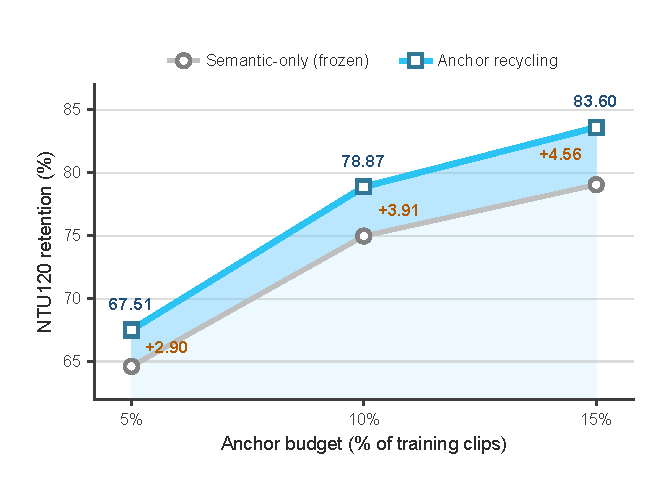
\includegraphics[width=0.72\linewidth]{fig3_budget_allocation.pdf}
\caption{Budget-allocation sweep on NTU120 at the 5\%, 10\%, and 15\%
budgets (Table~\ref{tab:budget}). The shaded ribbon is the anchor-recycling advantage; red
numbers give the gain in percentage points over the semantic-only arm.}
\label{fig:budget}
\end{figure}

\begin{quote}
\textbf{Finding 3.} The anchor-recycling advantage widens monotonically with budget. At
15\% the pipeline reaches 83.60\%, 1.4~pp below the PARTIAL band before
augmentation is applied; \S4.5 shows augmentation and a higher learning
rate lift the 10\% budget point past that band.
\end{quote}

\textbf{Matched-budget supervised baselines.} To test whether the recycling gain
is simply fine-tuning under another name, we train the same encoder
end-to-end on the same 10\% anchors (all parameters, same augmentation
family, BatchNorm statistics frozen). Full fine-tuning raises the
full-label reference from 58.37\% to 60.10\% but reaches only 80.32\%
retention, 4.87~pp below recycling (paired 95\% CI [4.29, 5.44]). It fits the
734 anchors almost perfectly (mean anchor accuracy 98.6\%), and the semantic
layer cannot harvest the resulting geometry. The comparison isolates the
mechanism: the constrained, distillation-anchored update is what preserves
label efficiency, not encoder adaptation per se. BitFit, which trains only
24,274 biases, reaches 76.02\% --- 1.06~pp above frozen and 9.14~pp below
recycling (paired 95\% CI [8.30, 10.01]) --- so the gap is not a parameter-count
effect either. A bottleneck Adapter (96,316 parameters) reaches 79.74\%,
still 5.42~pp below recycling (paired 95\% CI [3.91, 6.97]); the mean ordering
BitFit $<$ Adapter $<$ full fine-tuning $<$ recycling holds, with seed-level
variation in the middle two arms.

\begin{table}[t]
\centering
\caption{Matched-budget supervised baselines on NTU120 (10\% budget; ten
seeds).}
\label{tab:matched}
\small
\begin{tabular}{@{}lrrrr@{}}
\toprule
Arm & Trainable params & Retention & $\Delta$ vs.\ frozen & Full-label ref \\
\midrule
Frozen (semantic only) & 0 & 74.96\% & --- & 58.37\% \\
Full fine-tuning & 1.84\,M & 80.32\% & $+5.36$~pp & 60.10\% \\
BitFit (bias only) & 24,274 & 76.02\% & $+1.06$~pp & 60.06\% \\
Adapter (bottleneck) & 96,316 & 79.74\% & $+4.78$~pp & 58.30\% \\
Anchor recycling (LoRA) & 62,616 (3.19\%) & \textbf{85.16\%} & \textbf{$+10.20$~pp} & 58.24\% \\
\bottomrule
\end{tabular}
\end{table}

\subsection{Hyperparameter sensitivity}

On NTU120 (ten seeds per cell), only two factors matter. The adaptation
learning rate: 78.87\% (1e-3) $\rightarrow$ 82.13\% (1e-2) $\rightarrow$ 82.73\% (2e-2) without
augmentation; 4e-2 trips the calibration gate (\S4.6). The augmentation
multiplier: with lr 2e-2, 82.73\% ($\times 1$) $\rightarrow$ 83.41\% ($\times 4$) $\rightarrow$ \textbf{85.16\% ($\times 8$)} $\rightarrow$
84.38\% ($\times 12$), peaking at $\times 8$ (Figure~\ref{fig:dose}). Doubling the adaptation epochs from
100 to 200 yields 78.88\%, and removing the distillation weight entirely
yields 79.05\% at lr 1e-3, slightly above the 78.87\% obtained with $\lambda = 1$;
each variation moves the result by $\le 0.5$~pp. The LoRA rank shifts the result
more: at lr 1e-2, doubling the rank from 8 to 16 yields 81.49\%, versus
82.13\% for rank 8 at the same learning rate.

\begin{figure}[t]
\centering
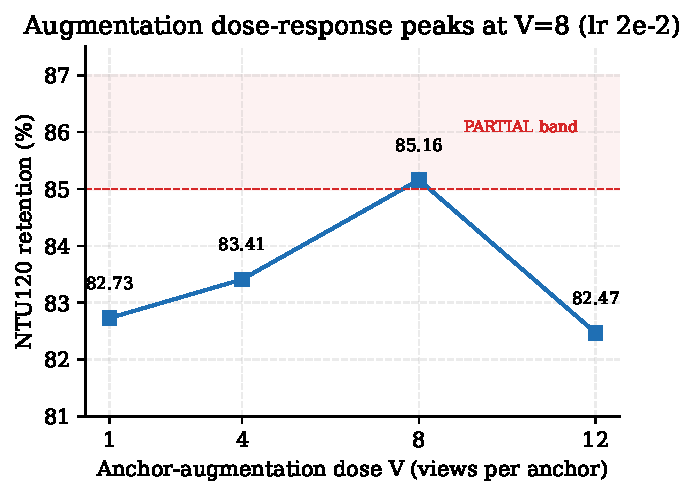
\includegraphics[width=0.72\linewidth]{fig4_aug_dose_response.pdf}
\caption{Effect of the augmentation multiplier on NTU120 at lr 2e-2. Boxes give the
interquartile range over ten seeds, dots individual seeds, and the coral line
the mean. The dashed line marks the 85\% PARTIAL threshold.}
\label{fig:dose}
\end{figure}

The optimal recipe differs across tiers in a way that tracks anchor mass:
NTU120 (734 anchors) takes the strongest setting (lr 2e-2, $8\times$ augmentation);
UCF101 (953 anchors) peaks at lr 2e-2 \emph{without} augmentation (71.21\%; the
augmented 1e-2 variant drops to 68.31\%); PanAf500 (40 anchors) needs the
gentlest setting (lr 1e-2, $4\times$ augmentation, 92.21\%) and breaks the gate at
2e-2 even with augmentation. UCF101, despite carrying the largest anchor
set, takes no augmentation: its video-derived reference is so weak (\S4.7)
that extra augmented views mostly add variance rather than usable signal, so
its recipe is governed by reference quality as much as by anchor mass.

\subsection{The envelope: anchor-mass floor and calibration-gate ceiling}

\textbf{Anchor-mass floor.} On PanAf500, naive recycling (40 anchors, batch 64)
produces \emph{zero} gradient steps and leaves all ten seeds bit-identical to the
frozen pipeline: the entire chain (features $\rightarrow$ clustering $\rightarrow$ pseudo-labels $\rightarrow$
predictions) reproduces exactly. With the batch handling fixed and
augmentation added at the gentle setting, the pipeline moves for the first
time and reaches CONFIRMS. In this naive, augmentation-free setting,
recycling is inert with the 40-anchor PanAf500 set and effective with the
734- and 953-anchor sets of NTU120 and UCF101; the transition between these
scales was not measured, and the anchor augmentation of \S3.2 is what lets
the 40-anchor PanAf500 set move at all.

\textbf{Calibration-gate ceiling.} When recycling pressure exceeds the envelope
(lr 4e-2 on NTU120; lr 2e-2 with augmentation on PanAf500), the semantic
layer's calibration gate selects $\tau = 0$ and the
pipeline raises a hard error rather than emitting degenerate pseudo-labels.
The gate converts silent quality collapse into an explicit, diagnosable
stop, and marks the ceiling of the adaptation envelope.

\begin{quote}
\textbf{Finding 4.} Anchor recycling lives in a two-sided envelope: an
anchor-mass floor beneath which unaugmented recycling is inert, and a
calibration-gate ceiling above which it stops in a hard, diagnosable error.
Both edges are reproducible and tier-dependent.
\end{quote}

\subsection{Threats to validity}

PanAf500's validation set is 25 clips, quantizing accuracies in 4\% steps; its
CONFIRMS verdict rests on 5/10 seeds improving, 3 tying, and 2 regressing
(sign test, not significant) plus a small reference drift (64.0\% $\rightarrow$ 61.6\%),
and should be interpreted with these quantification caveats in mind.
NTU120's PARTIAL margin is 0.16~pp above the band edge. UCF101's reference is
video-derived and weak (full-label linear reference $\approx 19\%$), so its retentions
are ratios of small numbers.

% =====================================================================
\section{Discussion}
% =====================================================================

\textbf{The mechanism behind recycling.} The negative-result study of \S4.2
isolates the mechanism by elimination: the label-free routes leave the
frozen geometry in place, cross-domain transfer improves features that the
semantic layer cannot harvest, and pseudo-label feedback entrenches the
inherited geometry. Recycling is the only arm whose supervision is real,
drawn from the target domain, and routed to the encoder. The k-ladder study ---
our prior budget sweep~\cite{prior} on the synthetic episode, which varied the anchor
count $k$ --- is consistent with this outcome: encoder quality responds to label
signal.

\textbf{The geometry--harvest mismatch.}
The cross-domain arm shows that absolute separability and retention can move
in opposite directions. The semantic layer's anchor clustering and confidence
gating are grown around a feature geometry; when the geometry changes faster
than the clustering, the discrete pipeline stages (cluster assignments,
pseudo-label acceptance, final predictions) may not flip at all. PanAf500's
bit-identical replication under naive recycling is the extreme case.
Recycling works because it moves the geometry \emph{gently} (low-rank,
distillation-anchored) and \emph{with} the semantic layer's own anchors, keeping
the two layers coherent during the update.

\textbf{Relation to full fine-tuning.} Prior controlled contrasts on the
synthetic taxonomy-transition benchmark of our earlier experiments~\cite{prior} show full
fine-tuning reaches 98.2\% while destroying the label-efficiency property it
is meant to serve. Recycling keeps 96.8\% of parameters frozen and preserves
the frozen inference path: it occupies the label-efficient point of the
adaptation spectrum rather than the accuracy-maximal one.

\textbf{The value of mapped negatives.} Each failed route is paired with a
mechanism: a statistics gap (TENT), saturation (continued pretraining), a
geometry--harvest mismatch (cross-domain), and label inheritance
(pseudo-label feedback). For
practitioners, the map indicates that in weak-reference regimes label-free
encoder adaptation is unlikely to pay off, and that the available labels are
better spent supervising both layers.

\textbf{Limitations.} Recycling is validated on skeleton data with GCN backbones
and LoRA-style convolution adapters; transfer to transformer encoders is
untested. The budget range studied is 5--15\%; we did not measure beyond it,
though we would expect much larger budgets to converge toward full
fine-tuning. PanAf500 and UCF101 verdicts carry the quantization
and weak-reference caveats of \S4.7. The calibration gate, while a useful
safety mechanism, is itself a hyperparameter surface we did not explore.

% =====================================================================
\section{Conclusion}
% =====================================================================

We studied the ceiling of decoupled skeleton behavior recognition in
weak-reference tiers and turned it into a method. A systematic negative-result
study shows that no label-free route (test-time adaptation, continued
self-supervised pretraining, cross-domain transfer, or pseudo-label feedback)
moves a frozen physical layer past its ceiling. The ceiling yields to a
simple idea: \textbf{recycle the same anchors that
drive the semantic layer as supervision for a low-rank physical-layer
update}. Across three weak-reference tiers this gains $+10.20$, $+9.71$, and
$+20.12$~pp and crosses two pre-registered verdict bands. The effect's
two-sided envelope (an anchor-mass floor for the naive recipe and a
calibration-gate ceiling) is mapped and released, along with every per-seed
number and the harness that produced them.

Beyond this paper, anchor recycling suggests a broader principle for
decoupled systems under evolving taxonomies: the labels that adapt the
decision layer can also be used to adapt the representation, provided the
update is kept within a magnitude the representation can absorb. Whether
this principle, and the boundary map that motivated it, extends to other
modalities where self-supervised physical encoders meet small, shifting,
expert-labeled semantic layers is a question we leave to future work.

% =====================================================================
% References
% =====================================================================
\begin{thebibliography}{99}

\bibitem{aimclr}
T.~Guo, H.~Liu, Z.~Chen, M.~Liu, T.~Wang, and R.~Ding, ``Contrastive
learning from extremely augmented skeleton sequences for self-supervised
action recognition,'' in \emph{Proc. AAAI Conf. Artificial Intelligence}, vol.~36,
2022, pp.~762--770.

\bibitem{crossclr}
L.~Li, M.~Wang, B.~Ni, H.~Wang, J.~Yang, and W.~Zhang, ``3D human action
representation learning via cross-view consistency pursuit,'' in \emph{Proc.
IEEE/CVF Conf. Computer Vision and Pattern Recognition (CVPR)}, 2021,
pp.~4739--4748.

\bibitem{hbehavemae}
L.~Stoffl, A.~Bonnetto, S.~d'Ascoli, and A.~Mathis, ``Elucidating the
hierarchical nature of behavior with masked autoencoders,'' in \emph{Proc.
European Conf. Computer Vision (ECCV)}, 2024, pp.~106--125.

\bibitem{treba}
F.~Sener, S.~Chakraborty, T.~Nandakumar, D.~Calogiuri, and A.~K.~Jain,
``TREBA: Using temporally-guided self-supervision for 3D human pose and
action recognition,'' in \emph{Proc. IEEE/CVF Winter Conf. Applications of
Computer Vision (WACV)}, 2023.

\bibitem{prosl}
H.~Qin, L.~Chen, M.~Kong, Z.~Zhao, X.~Zeng, M.~Lu, and Q.~Zhu,
``Progressive semantic learning for unsupervised skeleton-based action
recognition,'' \emph{Machine Learning}, vol.~114, no.~3, art.~64, 2025.

\bibitem{stgcn}
S.~Yan, Y.~Xiong, and D.~Lin, ``Spatial temporal graph convolutional
networks for skeleton-based action recognition,'' in \emph{Proc. AAAI Conf.
Artificial Intelligence}, 2018, pp.~7444--7451.

\bibitem{tent}
D.~Wang, E.~Shelhamer, S.~Liu, B.~Olshausen, and T.~Darrell, ``Tent: Fully
test-time adaptation by entropy minimization,'' in \emph{Proc. Int. Conf.
Learning Representations (ICLR)}, 2021.

\bibitem{lora}
Z.~Hu et al., ``LoRA: Low-rank adaptation of large language models,'' in
\emph{Proc. Int. Conf. Learning Representations (ICLR)}, 2022.

\bibitem{moco}
K.~He, H.~Fan, Y.~Wu, S.~Xie, and R.~Girshick, ``Momentum contrast for
unsupervised visual representation learning,'' in \emph{Proc. IEEE/CVF Conf.
Computer Vision and Pattern Recognition (CVPR)}, 2020.

\bibitem{simclr}
T.~Chen, S.~Kornblith, M.~Norouzi, and G.~Hinton, ``A simple framework
for contrastive learning of visual representations,'' in \emph{Proc. Int. Conf.
Machine Learning (ICML)}, 2020.

\bibitem{byol}
J.-B.~Grill et al., ``Bootstrap your own latent: A new approach to
self-supervised learning,'' in \emph{Proc. NeurIPS}, 2020.

\bibitem{ntu60}
A.~Shahroudy, J.~Liu, T.-T.~Ng, and G.~Wang, ``NTU RGB+D: A large scale
dataset for 3D human activity analysis,'' in \emph{Proc. IEEE Conf. Computer
Vision and Pattern Recognition (CVPR)}, 2016.

\bibitem{ntu120}
J.~Liu et al., ``NTU RGB+D 120: A large-scale benchmark for 3D human
activity understanding,'' \emph{IEEE Trans. Pattern Analysis and Machine
Intelligence}, vol.~42, no.~10, 2020.

\bibitem{ucf101}
K.~Soomro, A.~R.~Zamir, and M.~Shah, ``UCF101: A dataset of 101 human
action classes from videos in the wild,'' CRCV-TR-12-01, 2012.

\bibitem{panaf20k}
O.~Brookes et al., ``PanAf20K: A large video dataset for wild ape
detection and behaviour recognition,'' \emph{Int. J. Computer Vision}, vol.~132,
no.~8, pp.~3086--3102, 2024.

\bibitem{lwf}
Z.~Li and D.~Hoiem, ``Learning without forgetting,'' \emph{IEEE Trans. Pattern
Analysis and Machine Intelligence}, vol.~40, no.~12, 2018.

\bibitem{supcon}
P.~Khosla et al., ``Supervised contrastive learning,'' in \emph{Proc. NeurIPS},
2020.

\bibitem{rejection}
C.~Cortes, G.~DeSalvo, and M.~Mohri, ``Learning with rejection,'' in
\emph{Proc. Algorithmic Learning Theory (ALT)}, 2016, pp.~67--82.

\bibitem{dann}
Y.~Ganin and V.~Lempitsky, ``Unsupervised domain adaptation by backpropagation,''
in \emph{Proc. Int. Conf. Machine Learning (ICML)}, 2015.

\bibitem{bendavid}
S.~Ben-David et al., ``A theory of learning from different domains,''
\emph{Machine Learning}, vol.~79, 2010.

\bibitem{tta_distmatch}
W.~Wang, V.~W.~Zheng, H.~Liu, and L.~Zhou, ``Test-time adaptation with
distribution matching,'' 2022.

\bibitem{bituning}
X.~Peng and B.~Wang, ``Bi-tuning of pre-trained representations,'' 2022.

\bibitem{distillation}
G.~Hinton, O.~Vinyals, and J.~Dean, ``Distilling the knowledge in a neural
network,'' in \emph{NeurIPS Deep Learning Workshop}, 2015.

\bibitem{yosinski}
J.~Yosinski, J.~Clune, Y.~Bengio, and H.~Lipson, ``How transferable are
features in deep neural networks?'' in \emph{Proc. NeurIPS}, 2014.

\bibitem{alexnet}
A.~Krizhevsky, I.~Sutskever, and G.~Hinton, ``ImageNet classification with
deep convolutional neural networks,'' in \emph{Proc. NeurIPS}, 2012.

\bibitem{adamw}
I.~Loshchilov and F.~Hutter, ``Decoupled weight decay regularization,'' in
\emph{Proc. ICLR}, 2019.

\bibitem{adam}
D.~P.~Kingma and J.~Ba, ``Adam: A method for stochastic optimization,'' in
\emph{Proc. ICLR}, 2015.

\bibitem{dropout}
N.~Srivastava et al., ``Dropout: A simple way to prevent neural networks
from overfitting,'' \emph{JMLR}, vol.~15, 2014.

\bibitem{batchnorm}
S.~Ioffe and C.~Szegedy, ``Batch normalization: Accelerating deep network
training by reducing internal covariate shift,'' in \emph{Proc. ICML}, 2015.

\bibitem{resnet}
K.~He, X.~Zhang, S.~Ren, and J.~Sun, ``Deep residual learning for image
recognition,'' in \emph{Proc. CVPR}, 2016.

\bibitem{augmentation}
C.~Shorten and T.~M.~Khoshgoftaar, ``A survey on image data augmentation
for deep learning,'' \emph{J. Big Data}, 2019.

\bibitem{clip}
A.~Radford et al., ``Learning transferable visual models from natural
language supervision,'' in \emph{Proc. ICML}, 2021.

\bibitem{dinov2}
M.~Oquab et al., ``DINOv2: Learning robust visual features without
supervision,'' 2023.

\bibitem{multitask}
R.~Caruana, ``Multitask learning,'' \emph{Machine Learning}, vol.~28, 1997.

\bibitem{transfer_survey}
S.~J.~Pan and Q.~Yang, ``A survey on transfer learning,'' \emph{IEEE Trans.
Knowledge and Data Engineering}, vol.~22, no.~10, 2010.

\bibitem{entropy_min}
Y.~Grandvalet and Y.~Bengio, ``Semi-supervised learning by entropy
minimization,'' in \emph{Proc. NeurIPS}, 2005.

\bibitem{pseudolabel}
D.-H.~Lee, ``Pseudo-label: The simple and efficient semi-supervised
learning method for deep neural networks,'' in \emph{ICML Workshop}, 2013.

\bibitem{fixmatch}
K.~Sohn et al., ``FixMatch: Simplifying semi-supervised learning with
consistency and confidence,'' in \emph{Proc. NeurIPS}, 2020.

\bibitem{randomforest}
L.~Breiman, ``Random forests,'' \emph{Machine Learning}, vol.~45, no.~1,
2001, pp.~5--32.

\bibitem{sklearn}
F.~Pedregosa et al., ``Scikit-learn: Machine learning in Python,'' \emph{JMLR},
vol.~12, 2011.

\bibitem{prior}
(Authors of this paper), ``Physics--semantics decoupled skeleton behavior
recognition under evolving taxonomies,'' under review, 2026.

\end{thebibliography}

\clearpage
% Generated by scripts/p1_sprint/make_next_paper_appendix.py — do not edit by hand.
\appendix

\section{Tier construction and anchor draws}
\label{app:tiers}
\setcounter{table}{0}
\renewcommand{\thetable}{A.\arabic{table}}

All tiers pass through one export pipeline. Keypoints are resampled to
$T=30$, centered, and mapped to the 25-slot feeder consumed by the AimCLR
pretext. Human tiers use the COCO-17 to NTU25 map of
\texttt{export\_tier\_feeder.py}: the nose becomes the head slot, shoulders,
elbows, and wrists fill the six arm slots, hips, knees, and ankles fill the
six leg slots, and the hip root, spine mid, and neck are synthesized from
shoulder and hip means; slots 16--24 are zero. PanAf500 keypoints arrive in a
24-slot PSD24 layout produced by an AP-10K 17-keypoint animal pose model;
forelimbs map to the arm slots, hindlimbs to the leg slots, and the same
torso synthesis applies. The collected tiers therefore share one graph
topology, fixed at pretraining, and differ only in data and reference
quality. Anchor draws are stratified by class at 10\% of training clips per
seed (734, 953, and 40 anchors for the three headline weak-reference tiers;
1,200 for the 120-class replication), with seeds 42--51 throughout.

\begin{table}[H]
\centering
\caption{Tier construction. NTU60 is the published point of the prior study~\cite{prior}; the other tiers are re-run under the shared protocol.}
\label{tab:appA1}
\footnotesize
\begin{tabular*}{\textwidth}{@{\extracolsep{\fill}}lrrrrrr@{}}
\toprule
Tier & Classes & Train & Val & Anchors & Full ref (\%) & Frozen ret. (\%) \\
\midrule
NTU60 & 60 & — & — & — & 74.45 & 90.70 [41] \\
PanAf500 & 9 & 400 & 25 & 40 & 64.00 & 82.50 \\
NTU120 & 60 & 7,337 & 4,663 & 734 & 58.37 & 74.96 \\
UCF101 & 101 & 9,537 & 463 & 953 & 19.87 & 51.09 \\
NTU120-120c & 120 & 12,000 & 2,400 & 1,200 & 44.33 & 66.33 \\
NTU120-32ch & 60 & 7,337 & 4,663 & 734 & 56.85 & 68.48 \\
NTU120-64ch & 60 & 7,337 & 4,663 & 734 & 59.68 & 74.78 \\
\bottomrule
\end{tabular*}
\end{table}

NTU60 is not re-run in this paper; its row reports the published retention
of the prior study~\cite{prior} and serves as the strong-reference anchor
of the gradient.

\section{Zero-label adaptation suite}
\label{app:negative}
\setcounter{table}{0}
\renewcommand{\thetable}{B.\arabic{table}}

Table~\ref{tab:appB1} lists the five adaptation arms of \S4.2 and their
configurations. All arms receive the same 10\% anchor draw per seed and are
re-measured by the same three-arm protocol; no arm sees a label beyond the
anchor set, and the TENT, continued-pretraining, zero-shot, and cross-domain
arms see no labels at all.

\begin{table}[H]
\centering
\caption{Zero-label adaptation arms on NTU120 (10\% budget). All arms share the same anchor draws and the same three-arm measurement.}
\label{tab:appB1}
\footnotesize
\begin{tabular*}{\textwidth}{@{\extracolsep{\fill}}>{\raggedright\arraybackslash}p{5.0cm}>{\raggedright\arraybackslash}p{4.0cm}rr@{}}
\toprule
Arm (mechanism) & Key settings & Seeds & Retention (\%) \\
\midrule
Frozen baseline --- no adaptation & — & 42–51 & 74.96 \\
TENT --- entropy minimization over BN affine parameters & lr 1e-3, 1 step/batch, eval-statistics & 42–51 & 74.08 \\
Same-domain LoRA continued pretraining --- low-rank continued pretext on unlabeled target clips & 30 epochs, lr 1e-2, r 8, alpha 16, lambda 1.0 & 42–51 & 74.99 \\
Cross-domain zero-shot --- NTU60 source encoder, no target update & NTU60 phaseB epoch300 & 42–51 & 69.77 \\
Cross-domain LoRA transfer --- NTU60 source + low-rank update on target clips & 30 epochs, lr 1e-2, r 8, alpha 16 & 42–51 & 71.98 \\
Pseudo-label SupCon feedback --- encoder retrained on semantic-layer pseudo-labels & 1 round, 20 epochs, batch 256, lr 1e-3, tau 0.1, 7,239 labels & 42–51 & 74.98 \\
\bottomrule
\end{tabular*}
\end{table}

Table~\ref{tab:appB2} gives the per-seed (b)-arm accuracies behind
Table~\ref{tab:labelfree}. The frozen column is the semantic-only arm of
the frozen encoder; the remaining columns are the five adaptation arms. No
column crosses the 75\% line except the frozen baseline itself.

\begin{table}[H]
\centering
\caption{Per-seed (b)-arm accuracy (\%) behind Table~\ref{tab:labelfree}.}
\label{tab:appB2}
\scriptsize
\begin{tabular*}{\textwidth}{@{\extracolsep{\fill}}rrrrrrr@{}}
\toprule
Seed & Frozen & TENT & LoRA-CP & Zero-shot & LoRA-xfer & SupCon \\
\midrule
42 & 41.45 & 41.99 & 41.41 & 38.39 & 42.78 & 42.46 \\
43 & 43.94 & 43.90 & 42.98 & 38.99 & 42.87 & 43.11 \\
44 & 45.49 & 45.31 & 45.10 & 40.23 & 43.64 & 43.83 \\
45 & 42.33 & 42.74 & 42.70 & 38.11 & 41.93 & 43.02 \\
46 & 44.28 & 44.26 & 43.28 & 39.03 & 42.14 & 43.83 \\
47 & 43.23 & 43.06 & 43.06 & 37.32 & 42.53 & 43.38 \\
48 & 44.31 & 44.50 & 43.62 & 39.72 & 43.43 & 43.43 \\
49 & 44.41 & 44.22 & 43.62 & 40.68 & 42.44 & 41.78 \\
50 & 43.66 & 43.06 & 43.08 & 37.27 & 42.76 & 43.53 \\
51 & 44.43 & 44.28 & 44.54 & 39.59 & 44.95 & 43.53 \\
\bottomrule
\end{tabular*}
\end{table}

Two diagnostics complete the picture. First, a naive TENT configuration that
adapts in BatchNorm train mode collapses the 10\% head from 44\% to 27.0\%;
the collapse is a train/evaluation statistics artifact, and once the
statistics contract is fixed the same arm moves retention by only
$-0.88$~pp. Second, cross-domain LoRA transfer produces the highest absolute
separability of any arm (full-label reference 59.66\% and 10\% linear head
45.27\%, both above the frozen 58.37\%/44.18\%), yet its retention falls to
71.98\%: the semantic layer cannot harvest the improved geometry.

\section{Recycling per-seed results and hyperparameter grid}
\label{app:grid}
\setcounter{table}{0}
\renewcommand{\thetable}{C.\arabic{table}}

Table~\ref{tab:appC1} lists the per-seed retention of the three headline
recycling configurations. Every NTU120 seed improves; PanAf500 improves on
five seeds, ties on three, and regresses on two (the quantization caveat of
\S4.8); UCF101 improves on nine of ten seeds (one seed regresses by
1.94~pp).

\begin{table}[H]
\centering
\caption{Per-seed retention (\%) of the three headline recycling configurations.}
\label{tab:appC1}
\small
\begin{tabular*}{\textwidth}{@{\extracolsep{\fill}}rrrr@{}}
\toprule
Seed & NTU120 (lr 2e-2, $\times 8$) & PanAf500 (lr 1e-2, $\times 4$) & UCF101 (lr 2e-2) \\
\midrule
42 & 85.40 & 93.75 & 81.40 \\
43 & 84.33 & 107.14 & 60.00 \\
44 & 85.07 & 76.47 & 71.43 \\
45 & 87.57 & 58.33 & 98.75 \\
46 & 87.35 & 92.86 & 52.27 \\
47 & 84.95 & 100.00 & 65.59 \\
48 & 85.44 & 106.25 & 80.43 \\
49 & 84.55 & 94.12 & 62.65 \\
50 & 84.06 & 93.33 & 63.11 \\
51 & 83.09 & 94.12 & 82.50 \\
\bottomrule
\end{tabular*}
\end{table}

Per-seed retention is the ratio of the seed's (b)-arm accuracy to its own
full-label reference and can exceed 100\% when the (b) arm beats that
reference on a seed; the headline number is the ratio of means.

Bootstrap of the ratio of means (10,000 resamples over seeds) gives $95\%$ confidence intervals of +10.21~pp [+9.44, +11.06] on NTU120, +9.68~pp [+1.27, +16.25] on PanAf500, +20.17~pp [+12.73, +28.24] on UCF101, and +10.82~pp [+9.49, +12.31] on the 120-class replication, and +15.07~pp [+13.63, +16.60] on the 32-channel capacity control, and +8.84~pp [+8.16, +9.49] on the standard-width (64-channel) control. The per-seed sign tests are 10/0/0 ($p=0.002$), 5/3/2 ($p=0.453$), 9/0/1 ($p=0.022$), and 10/0/0 ($p=0.002$) on the 120-class replication, 10/0/0 ($p=0.002$) on the capacity control, and 10/0/0 ($p=0.002$) on the standard-width control; PanAf500's sign test is not significant, so its CONFIRMS verdict is descriptive rather than a significance claim. In raw (b)-arm accuracy the corresponding intervals are +5.85~pp [+5.04, +6.72], +4.00~pp [-2.40, +10.80], +3.63~pp [+2.03, +5.14], and +3.65~pp [+2.99, +4.40] on the 120-class replication, +12.27~pp [+11.40, +13.17] on the capacity control, and +7.68~pp [+7.06, +8.32] on the standard-width control. On the class-addition episode (60->120; Table 8 of the main text) the raw gain is +5.20~pp [+4.70, +5.68], the new-class gain is +7.57~pp [+7.10, +8.05], the retention gain is +15.49~pp [+14.54, +16.55] under the own-denominator convention (+12.11~pp [+10.94, +13.22] under a frozen denominator), and the old-class forgetting is reduced by 2.84~pp [2.03, 3.53]; all sign tests are 10/0/0 ($p=0.002$).

Table~\ref{tab:appC2} gives the full NTU120 sensitivity grid. The
augmentation rows use 50 epochs and the no-augmentation rows 100 epochs, as
in the main text; every cell uses ten seeds. The lr 4e-2 cell terminates at
the calibration gate (\ref{app:gate}) and therefore has no
retention value.

\begin{table}[H]
\centering
\caption{NTU120 sensitivity grid (ten seeds per cell; augmentation rows use 50 epochs, no-augmentation rows 100).}
\label{tab:appC2}
\footnotesize
\begin{tabular*}{\textwidth}{@{\extracolsep{\fill}}lrrrrrrl@{}}
\toprule
Configuration & lr & $V$ & Epochs & $\lambda$ & Rank & Retention (\%) & Verdict \\
\midrule
lr 1e-3 & 1e-3 & 1 & 100 & 1.0 & 8 & 78.87 & FAILS \\
lr 1e-2 & 1e-2 & 1 & 100 & 1.0 & 8 & 82.13 & FAILS \\
lr 2e-2 & 2e-2 & 1 & 100 & 1.0 & 8 & 82.73 & FAILS \\
lr 4e-2 & 4e-2 & 1 & 100 & 1.0 & 8 & gate & tau = 0 \\
aug x4 & 2e-2 & 4 & 50 & 1.0 & 8 & 83.41 & FAILS \\
aug x8 & 2e-2 & 8 & 50 & 1.0 & 8 & 85.16 & PARTIAL \\
aug x12 & 2e-2 & 12 & 50 & 1.0 & 8 & 84.38 & FAILS \\
aug x4, lr 1e-2 & 1e-2 & 4 & 50 & 1.0 & 8 & 82.06 & FAILS \\
epochs 200 & 1e-3 & 1 & 200 & 1.0 & 8 & 78.88 & FAILS \\
no distillation & 1e-3 & 1 & 100 & 0.0 & 8 & 79.05 & FAILS \\
rank 16 & 1e-2 & 1 & 100 & 1.0 & 16 & 81.49 & FAILS \\
\bottomrule
\end{tabular*}
\end{table}

Table~\ref{tab:appC3} gives the per-seed detail of the 120-class scale
replication. Every seed improves in both raw (b)-arm accuracy and retention;
per-seed retention ranges from 74.39\% to 82.61\%.

\begin{table}[H]
\centering
\caption{Per-seed detail of the 120-class scale replication (ten seeds).}
\label{tab:appC3}
\small
\begin{tabular*}{\textwidth}{@{\extracolsep{\fill}}rrrr@{}}
\toprule
Seed & Frozen b-arm (\%) & Recycling b-arm (\%) & Recycling retention (\%) \\
\midrule
42 & 29.71 & 32.46 & 77.51 \\
43 & 29.79 & 33.75 & 77.51 \\
44 & 28.75 & 35.04 & 82.61 \\
45 & 28.96 & 33.17 & 74.74 \\
46 & 30.29 & 33.21 & 76.20 \\
47 & 28.63 & 31.58 & 74.39 \\
48 & 28.96 & 32.92 & 77.91 \\
49 & 29.04 & 33.50 & 78.21 \\
50 & 29.46 & 31.46 & 74.60 \\
51 & 30.50 & 33.46 & 78.11 \\
\bottomrule
\end{tabular*}
\end{table}

Table~\ref{tab:appC4} repeats the per-seed detail for the 32-channel
capacity control. Every seed improves in retention; the frozen b-arm mean is
38.93\% and the recycled
mean is 51.20\%.

\begin{table}[H]
\centering
\caption{Per-seed detail of the 32-channel capacity control (ten seeds).}
\label{tab:appC4}
\small
\begin{tabular*}{\textwidth}{@{\extracolsep{\fill}}rrrr@{}}
\toprule
Seed & Frozen b-arm (\%) & Recycling b-arm (\%) & Recycling retention (\%) \\
\midrule
42 & 38.43 & 51.19 & 83.23 \\
43 & 38.45 & 49.86 & 81.07 \\
44 & 40.51 & 51.75 & 83.49 \\
45 & 39.27 & 52.80 & 85.99 \\
46 & 38.75 & 53.40 & 85.57 \\
47 & 37.16 & 50.65 & 84.78 \\
48 & 39.67 & 53.23 & 87.89 \\
49 & 39.67 & 50.40 & 82.43 \\
50 & 38.88 & 49.05 & 79.80 \\
51 & 38.54 & 49.65 & 81.29 \\
\bottomrule
\end{tabular*}
\end{table}

Table~\ref{tab:appC5} repeats the per-seed detail for the standard-width
(64-channel) control. Every seed improves in retention; the frozen b-arm mean
is 44.63\% and the
recycled mean is 52.31\%.

\begin{table}[H]
\centering
\caption{Per-seed detail of the standard-width (64-channel) control (ten seeds).}
\label{tab:appC5}
\small
\begin{tabular*}{\textwidth}{@{\extracolsep{\fill}}rrrr@{}}
\toprule
Seed & Frozen b-arm (\%) & Recycling b-arm (\%) & Recycling retention (\%) \\
\midrule
42 & 43.92 & 51.02 & 82.58 \\
43 & 45.04 & 52.58 & 84.35 \\
44 & 45.10 & 53.40 & 85.27 \\
45 & 45.04 & 53.42 & 84.67 \\
46 & 43.64 & 53.44 & 84.05 \\
47 & 44.35 & 51.96 & 84.13 \\
48 & 44.61 & 52.73 & 84.21 \\
49 & 44.35 & 51.36 & 82.70 \\
50 & 44.74 & 51.88 & 81.97 \\
51 & 45.51 & 51.30 & 82.26 \\
\bottomrule
\end{tabular*}
\end{table}

Table~\ref{tab:appC6} gives the per-seed detail of the class-addition
episode (60->120; old anchors stay spent). Forgetting is the phase-1
old-class accuracy minus the phase-2 old-class accuracy.

\begin{table}[H]
\centering
\caption{Per-seed detail of the class-addition episode (60->120; old anchors stay spent). P1 old = phase-1 old-class accuracy (\%); Sem./Rec.\ all = phase-2 overall accuracy (\%); New = new-class accuracy (\%); Fgt. = old-class forgetting in pp (phase-1 minus phase-2).}
\label{tab:appC6}
\scriptsize
\begin{tabular*}{\textwidth}{@{\extracolsep{\fill}}rrrrrrrr@{}}
\toprule
Seed & P1 old & Sem. all & Rec. all & New sem. & New rec. & Fgt. sem. & Fgt. rec. \\
\midrule
42 & 44.17 & 28.21 & 32.25 & 22.17 & 30.00 & 9.92 & 9.67 \\
43 & 41.50 & 25.54 & 29.50 & 21.25 & 27.75 & 11.67 & 10.25 \\
44 & 42.33 & 26.50 & 32.46 & 20.75 & 29.00 & 10.08 & 6.42 \\
45 & 43.08 & 27.62 & 32.21 & 22.58 & 30.17 & 10.42 & 8.83 \\
46 & 41.58 & 27.17 & 33.37 & 22.83 & 31.75 & 10.08 & 6.58 \\
47 & 42.50 & 28.33 & 33.87 & 25.00 & 32.58 & 10.83 & 7.33 \\
48 & 43.92 & 26.96 & 32.08 & 23.00 & 30.00 & 13.00 & 9.75 \\
49 & 41.25 & 28.00 & 33.37 & 23.50 & 30.58 & 8.75 & 5.08 \\
50 & 43.83 & 26.67 & 32.92 & 22.50 & 30.92 & 13.00 & 8.92 \\
51 & 44.75 & 28.08 & 33.08 & 22.67 & 29.17 & 11.25 & 7.75 \\
\bottomrule
\end{tabular*}
\end{table}

\section{Calibration-gate failure cases}
\label{app:gate}

The calibration gate turns a silent quality collapse into an explicit
error. Three configurations exceed the adaptation envelope and all stop in
the same place. On NTU120 at lr 4e-2, the anchor objective never leaves
chance: the loss stays at 5.10 for 100 epochs and the anchor accuracy ends
at 1.7\% over 60 classes. On PanAf500 at lr 2e-2 with $4\times$
augmentation, the anchor objective does fit (loss 5.51 to 1.75, anchor
accuracy 35.7\% over 9 classes), but the adapted feature geometry still
drives the selected similarity threshold to zero. In the 32-channel capacity
control, the 16-channel-optimal recipe (lr 2e-2, $8\times$ augmentation)
completes five seeds and trips on the sixth (seed 47): the anchor objective
stays at chance (loss 5.10, anchor accuracy 1.7\% over 60 classes). In all
cases the semantic
stage raises \texttt{ValueError} with the message
``tau must be positive: 0.0'' from the
threshold constructor before any pseudo-label is emitted.

The three cases are complementary. The first shows a gate trip caused by an
objective that never converged; the second shows a gate trip caused by a
converged objective whose geometry is nevertheless incompatible with the
semantic layer's calibration. The third shows that the upper edge moves with
encoder width: the recipe that is stable at 16 channels is too strong at 32,
so the capacity control uses lr 1e-2, where all ten seeds pass. A
training-loss monitor alone would have
accepted the second run. The gate is therefore not a duplicate of the
training objective but an independent check on the feature geometry that the
next stage will actually consume.

\section{Reproduction}
\label{app:repro}

The three-arm measurement is implemented once, in
\path{labelfree_tier_replication.py} (\texttt{run\_arms}), and reused
by every table: arm (a) fits a linear head on the $b$\% anchors; arm (b) runs
the semantic pipeline on the same anchors; arm (c) fits the full-label
linear reference on the same frozen features. The recycling driver
\path{t4_budget_split_tier.py} performs, per seed, the LoRA update on
that seed's anchors, re-exports the features, and re-runs the same three
arms, so the denominator always reflects the encoder actually measured.

{\footnotesize
\begin{verbatim}
# 1) feeder export (T=30, 25-slot map)
python scripts/p1_sprint/export_tier_feeder.py \
  --tier ntu120

# 2) frozen label-free pretext and three-arm readout
python scripts/p1_sprint/labelfree_tier_replication.py \
  --tier ntu120 --seeds 10

# 3) anchor recycling (tag fixes the summary name)
python scripts/p1_sprint/t4_budget_split_tier.py \
  --tier ntu120 --arm same10 --seeds 10 --epochs 100 \
  --lr 0.02 --aug-views 8 --tag aug8_lr2e2

# 4) label-free baselines
python scripts/p1_sprint/tta_tent_tier.py \
  --tier ntu120 --seeds 10 --bn-mode eval
python scripts/p1_sprint/lora_continue_tier.py \
  --tier ntu120 --epochs 30 --lr 0.01 \
  --source-ckpt runs/p1_sprint/labelfree_ntu120/pretext/epoch150_model.pt
python scripts/p1_sprint/supcon_feedback_tier.py \
  --tier ntu120 --rounds 1 --epochs 20 --psd-seed 42

# 5) 120-class scale replication (balanced 120 x 100/20, fresh pretext)
python scripts/p1_sprint/export_tier_feeder.py \
  --tier ntu120_full
python scripts/p1_sprint/labelfree_tier_replication.py \
  --tier ntu120_full --seeds 10
python scripts/p1_sprint/t4_budget_split_tier.py \
  --tier ntu120_full --arm same10 --seeds 10 --epochs 50 \
  --lr 0.02 --aug-views 8 --tag full10

# 6) 32-channel capacity control (same feeder via directory junction)
python scripts/run_ntu_phaseb.py \
  --config configs/labelfree_ntu120_32ch_pretext.yaml
python scripts/p1_sprint/labelfree_tier_replication.py \
  --tier ntu120_32ch --seeds 10
python scripts/p1_sprint/t4_budget_split_tier.py \
  --tier ntu120_32ch --arm same10 --seeds 10 --epochs 50 \
  --lr 0.01 --aug-views 8 --tag aug8_lr1e2

# 7) standard-width (64-channel) control
python scripts/run_ntu_phaseb.py \
  --config configs/labelfree_ntu120_64ch_pretext.yaml
python scripts/p1_sprint/labelfree_tier_replication.py \
  --tier ntu120_64ch --seeds 10
python scripts/p1_sprint/t4_budget_split_tier.py \
  --tier ntu120_64ch --arm same10 --seeds 10 --epochs 50 \
  --lr 0.01 --aug-views 8 --tag aug8_lr1e2

# 8) class-addition taxonomy episode (60 -> 120)
python scripts/p1_sprint/taxonomy_addition_recycle.py \
  --seeds 10 --epochs 50 --lr 0.02 --aug-views 8 --tag add60to120
\end{verbatim}
}

Checkpoints: the frozen pretexts are
\path{runs/p1_sprint/labelfree_<tier>/pretext/epoch150_model.pt}; the
NTU60 source used by the cross-domain arms is
\path{runs/ntu_phaseB/joint_pretext/epoch300_model.pt}; the released
adapted checkpoints are
\path{adapt_lora_xfer_ntu120/lora_epoch30_model.pt} and
\path{adapt_supcon_ntu120/supcon_r1_epoch20_model.pt}. Every summary
JSON carries its seeds, per-seed rows, configuration, and wall-clock time;
the evidence mirror under \path{reports/p1_sprint_evidence/} is
byte-identical to the run outputs.


\end{document}
